\chapter{El reloj de Sol -- III}
\label{sec:el-reloj-de-sol-iii}

% \setlength{\epigraphwidth}{0.5\textwidth}
% \epigraph{La optimización prematura es la raíz de todos los males en
%   computación.}
%    {\textsc{Atribuido a Donald Knuth, C.A.R. Hoare y Edsger Dijkstra
%    hacia 1970 (aunque probablemente sea parte del folclore
%    informático).}}


\hfill%
\begin{minipage}[]{.60\linewidth}
\begin{flushright}
  \emph{La optimización prematura es la raíz de todos los males en
    computación.}\footnotemark
\end{flushright}
\end{minipage}
\footnotetext{Atribuido a Donald Knuth, C.A.R. Hoare y Edsger Dijkstra
  hacia 1970 (aunque probablemente haya sido parte del folclore
  informático desde siempre).}

\vspace{4ex} \lettrine[lines=2]{E}{l Sol, asomado} a la ventana de la
oficina de Antonia, encontró bien temprano a nuestras protagonistas
sentadas frente a la siempre dócil computadora.

Cecilia se sentía tan cerca de terminar el reloj que casi no era capaz
de disfrutar de la felicidad que ---no lo dudaba--- debía
embargarla. Su estado le recordaba las ocaciones en que se encontraba
``pasada de sueño'' después de una larga noche en vela, al extremo de
no sentir ya ganas de dormir.

---Ahora sí... ¡Atravesemos nuestro reloj con todas las horas del día!
---exclamó, procurando sonar festiva y radiante.

%\begin{center}
%\begin{minipage}[]{.55\textwidth}%\vspace{0pt}
 \begin{lstlisting}
module reloj_de_sol(){
  difference(){
    cuerpo(largo_reloj);    
    hora_solar(6,20);
    hora_solar(6,40);
    for(hora=[7:17],
        minuto=[0,20,40])
          hora_solar(hora,minuto);
  }
}
reloj_de_sol();
 \end{lstlisting}%
 % \end{minipage}\hfill
% \begin{center}
%   % \begin{minipage}[]{.45\textwidth}%\vspace{0pt}
%    %    \centering
%   \includegraphics[width=.6\textwidth]{reloj-completo-no-optimizado}
% %\end{minipage}
% \end{center}

 Cecilia releyó su texto no sin orgullo. Debía horadar el reloj con
 las horas comprendidas entre las 6:20 y las 17:40, a intervalos de 20
 minutos. Para eso creó un bucle doble en las líneas 6 y 7: el primero
 recorría las horas desde las 7 hasta las 17 mientras que el segundo
 debía ofrecer los minutos 0, 20 y 40, por lo que no tenía sentido
 escribir un rango: con un simple vector explícito bastaba. Las 6:20 y
 las 6:40 hubieran sido difíciles de incluir en el bucle: consideró
 más económico expresarlas por separado en las líneas 4 y 5.

\begin{figure}[ht]
  \centering
  \includegraphics[width=.85\textwidth]{imagenes/reloj-completo-no-optimizado}
  \caption{Primera versión del reloj de Sol digital.}
  \label{fig:reloj-completo-no-optimizado}
\end{figure}


La vista previa, con \keystroke{F5}, fue prácticamente instantánea: en
la computadora de Antonia demandó apenas 0,166 segundos. Pero Cecilia
sabía que para poder imprimir el reloj era necesario compilarlo con la
más exigente \keystroke{F6}: sólo tras casi 10 minutos, y con los
ventiladores del procesador aullando a toda velocidad, el Intel i7 de
8\sptext{va} generación con 32 GB de RAM fue capaz de desplegar
finalmente frente a sus ojos el tan largamente ansiado reloj.

Cecilia, una vez más a lo largo de este manual, giró sobre sí misma
para compartir con Antonia su emoción, que ahora sí se abría paso
sensiblemente en su pecho a la vista del reloj terminado. Pero, como
también ocurriera tantas otras veces, encontró a Antonia con un gesto
de reserva y contemplando con ojos críticos el resultado y el
texto. Cecilia supo inmediatamente que este capítulo distaba mucho de
estar concluido:

---¿Y ahora qué? ---preguntó lacónicamente y con desgano.

Antonia salió rápidamemente de su ensimismamiento:

---¡No te pongas así! ---bromeó, riendo---. Por supuesto que así como
está podemos darnos por satisfechas, y mandarlo a imprimir. Sin
embargo... ¿Puede una artista dar alguna vez por concluida su obra?
---preguntó con aire retórico.

Cecilia no se sentía una artista: sólo quería terminar el
reloj. Además, recordó con terror que algunos pintores llegaron a
afirmar que vendían sus obras sólo para no pasarse la vida
retocándolas: ¿Pretendería Antonia que este manual durara tanto
tiempo?  Porque no se imaginaba vendiendo relojes de Sol
digitales... Tras un instante, decidió sin embargo desechar esos
temores y confiar en su amiga como hasta ahora, por lo que con la
mirada la invitó a continuar.

\section{Optimización}


Antonia parecía buscar la mejor manera de comenzar; tal vez cediendo a
su pulsión docente, lo hizo una vez más con una pregunta:

---¿Cuántos dígitos aparecen en la posición de las unidades de los
minutos?

Cecilia se sintió obligada a responder:

---Pues... uno solo: el cero, por supuesto ---y ni bien terminó la
frase, sintió que un asomo de comprensión empezaba a iluminarla de
manera difusa pero clara.

---O sea que desde las 6:20 hasta las 17:40 ese último dígito será
siempre y constantemente `0', ¿no? ---era evidente que Antonia trataba
de dotar estas preguntas de un tono de neutra ingenuidad.

---Claro... ---respondió lentamente Cecilia, procurando con todas sus
fuerzas hacer surgir y dar cuerpo a la incipiente idea que pugnaba por
aflorar en su conciente.

---¡Qué lástima tener que usar tantos rayos para un sólo dígito
repetido...! ---el lamento de Antonia no podía ser más sobreactuado;
Cecilia casi empezaba a ponerse nerviosa:

---¿Proponés que atravesemos el cero con un solo rayo?
---pre\-gun\-tó, más para ver si conseguía de Antonia que revelara su
secreto que por otra razón.

Antonia, por toda respuesta, simplemente se alzó de hombros y simuló
un gesto de perplejidad poco convincente.

Cecilia, tras unos momentos de intensa reflexión con la mirada vuelta
hacia el monitor, finalmente se dio por vencida:

---Ok, Antonia... ¿Qué es lo que proponés?

\section{Un haz de rayos de Sol}

Antonia tomó el teclado con resignación; era evidente que le hubiera
gustado que Cecilia resolviera por su cuenta el enigma. Como tantos
otros docentes, era injusta: pretendía que los demás resolvieran en
pocos segundos cuestiones que a ellos les habían demandado semanas,
cuando no meses.

---¿Te acordás cuando empezamos a escribir nuestro rayo de Sol, allá
por el capítulo \ref{cap:el-primer-rayo-de-sol-i}? ---evocó, mientras
desplegaba en el monitor los diagramas que copiamos en la figura
\ref{fig:poligonos-auxiliares}.


\begin{figure}[t]
  \centering
  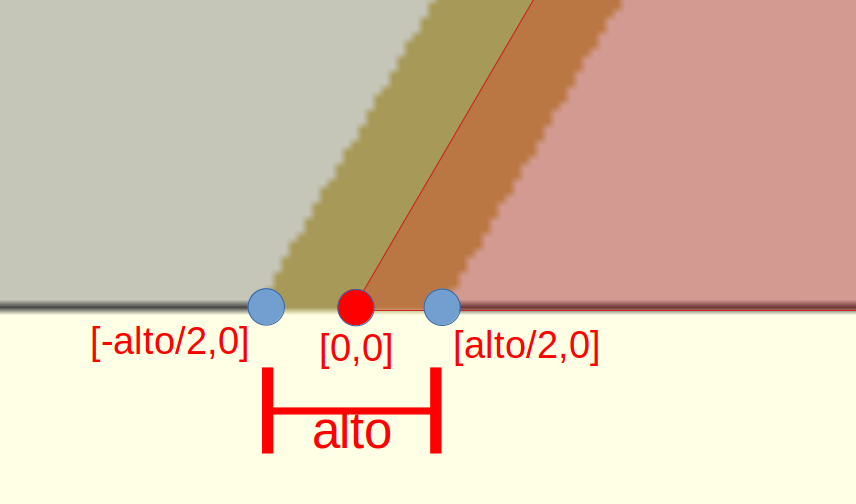
\includegraphics[width=.55\textwidth]{imagenes/poligono-puntos-base}\hfill
  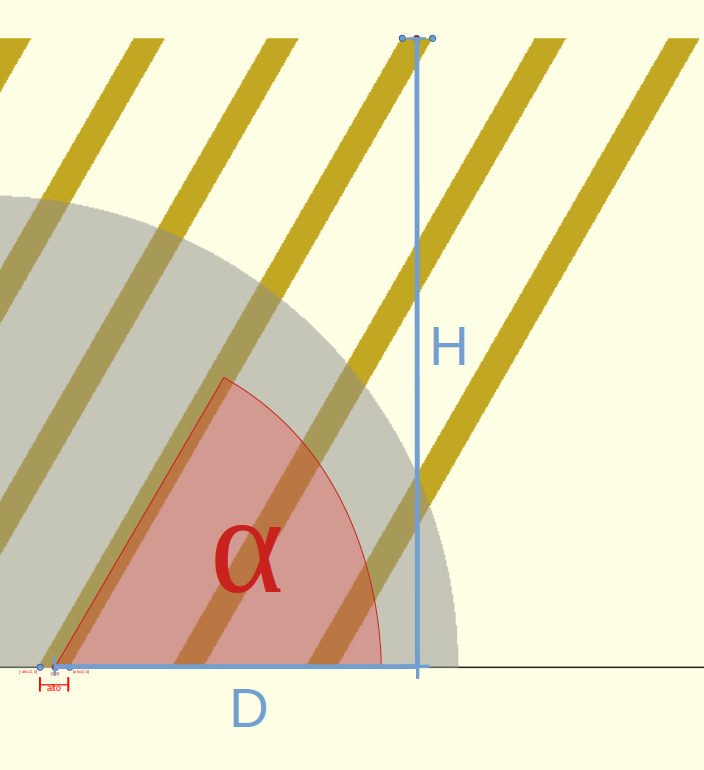
\includegraphics[width=.44\textwidth]{imagenes/poligono-tangente}  
  \caption{Gráficos auxiliares para la determinación de los extremos
    de cada rayo de Sol.}
  \label{fig:poligonos-auxiliares}
\end{figure}

Cecilia lo recordaba perfectamente: esos diagramas les habían
permitido expresar las coordenadas de los vértices de cada rayo:
\texttt{[-alto/2,0], [D-alto/2,H], [D+alto/2,H], [alto/2,0]}.

---Supongamos que sabemos que un mismo dígito existe entre dos horas
distintas, que se corresponden a dos ángulos diferentes: digamos,
$\alpha_1$ y $\alpha_2$ ---propuso cautamente Antonia, señalando la
figura \ref{fig:dos-rayos-alfas}.


\begin{figure}[ht]
  \centering
  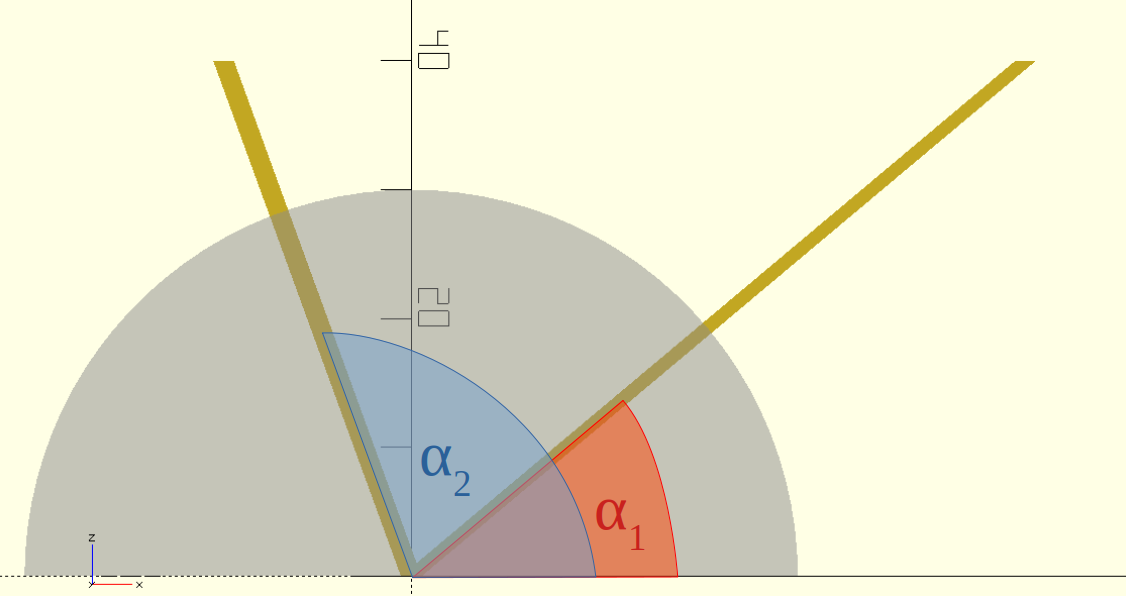
\includegraphics[width=.65\textwidth]{imagenes/dos-rayos-alfas}  
  \caption{Dos rayos solares con distintas inclinaciones, que Antonia
    propone que pueden ser los extremos de un mismo dígito presente
    entre dos horas distintas.}
  \label{fig:dos-rayos-alfas}
\end{figure}


\guillemotright ¿Deberemos trazar \emph{tooodos} los rayos entre
ambos extremos..?  ---la manera en que arrastró las oes era una de las
peores costumbres de Antonia como docente, pero a Cecilia casi no la
molestó: ya sentía que la comprensión se abría paso con más seguridad
en su mente.


\begin{figure}[ht]
  \centering
  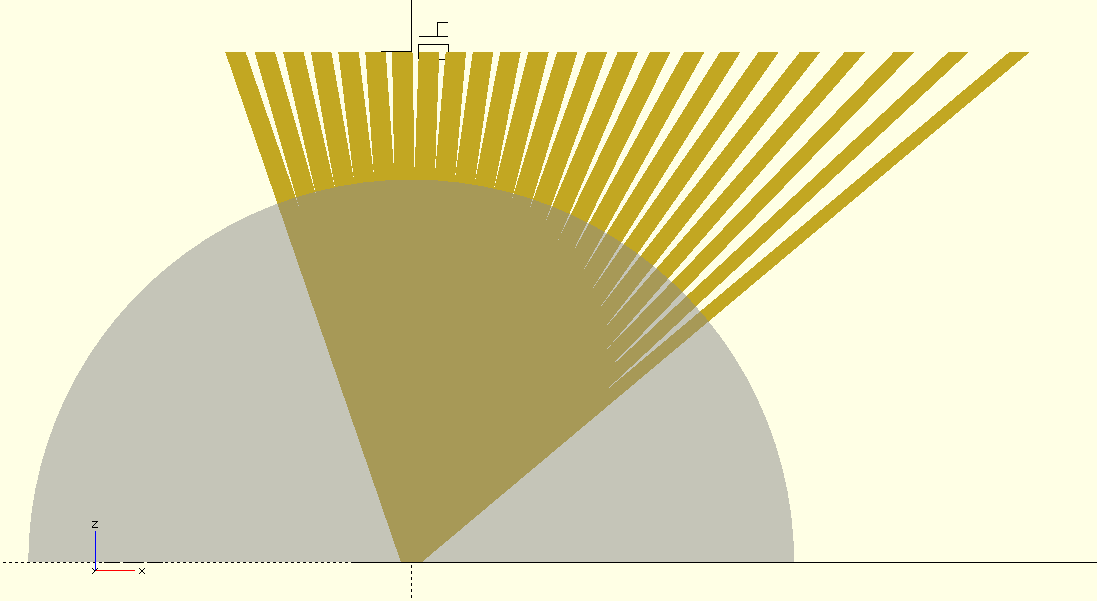
\includegraphics[width=.6\textwidth]{imagenes/muchos-rayos}  
  \caption{Antonia despliega los muchos rayos que deberían
    corresponderse con un sólo dígito que persistiera entre dos horas
    distintas.}
  \label{fig:muchos-rayos}
\end{figure}


---¿Vos decís que reemplacemos todos los rayos por un único haz?
---aventuró Cecilia.

---¡Sí! ---gritó triunfalmente Antonia, queriendo creer que su amiga
ya había desentrañado el misterio del to\-\mbox{do---.} Fijate que cada rayo lo
creamos como un polígono. Si bien nosotras venimos trabajando con
ellos como si fueran necesariamente paralelogramos, nada cuesta
reemplazar los vértices superiores de un solo rayo para convertirlo en
un suficiente haz.


\begin{figure}[ht]
  \centering
  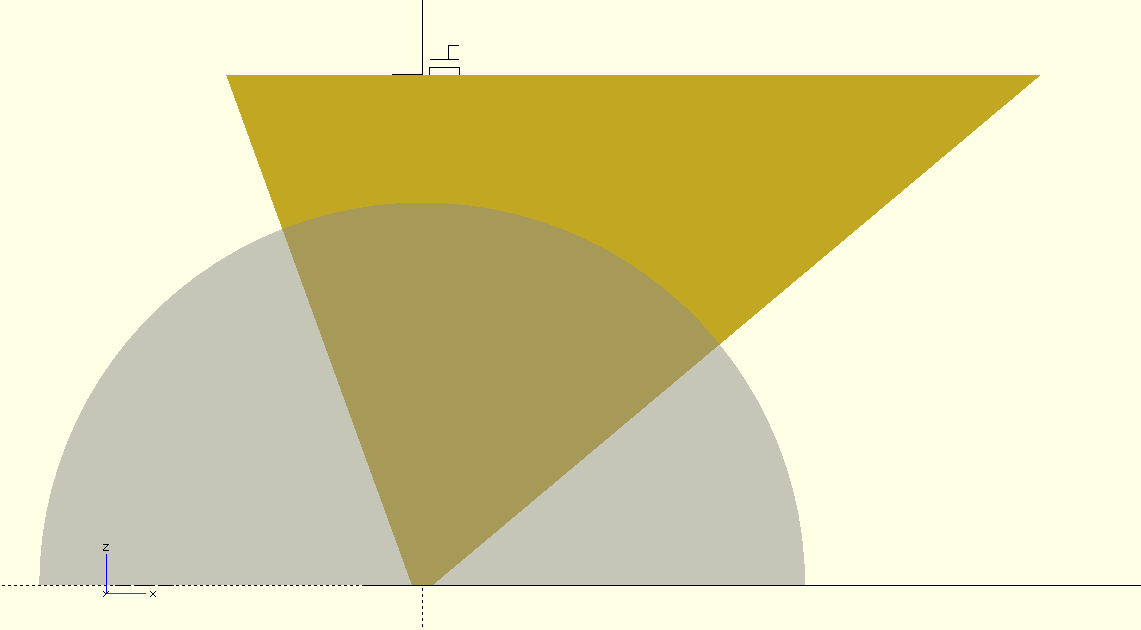
\includegraphics[width=.6\textwidth]{imagenes/haz}
  \caption{Haz de rayos de Sol, desplegados entre dos horas extremas.}
  \label{fig:haz}
\end{figure}


A Cecilia le gustó la propuesta expresada en la figura \ref{fig:haz},
y la idea ---al menos como aspiración--- le parecía cada vez más
hermosa, si bien debía admitir para sus adentros que todavía no
acababa de entenderla del todo.

---Para calcular los vértices superiores del haz que buscamos sólo
debemos remitirnos a los correspondientes de los rayos extremos
---siguió Antonia, quizá con demasiada velocidad. Ése era otro de sus
vicios docentes preferidos: pasaba de una lentitud exasperante a una
velocidad vertiginosa sin demostrar piedad alguna por sus
circunstanciales alumnos.


\begin{figure}[ht]
  \centering
  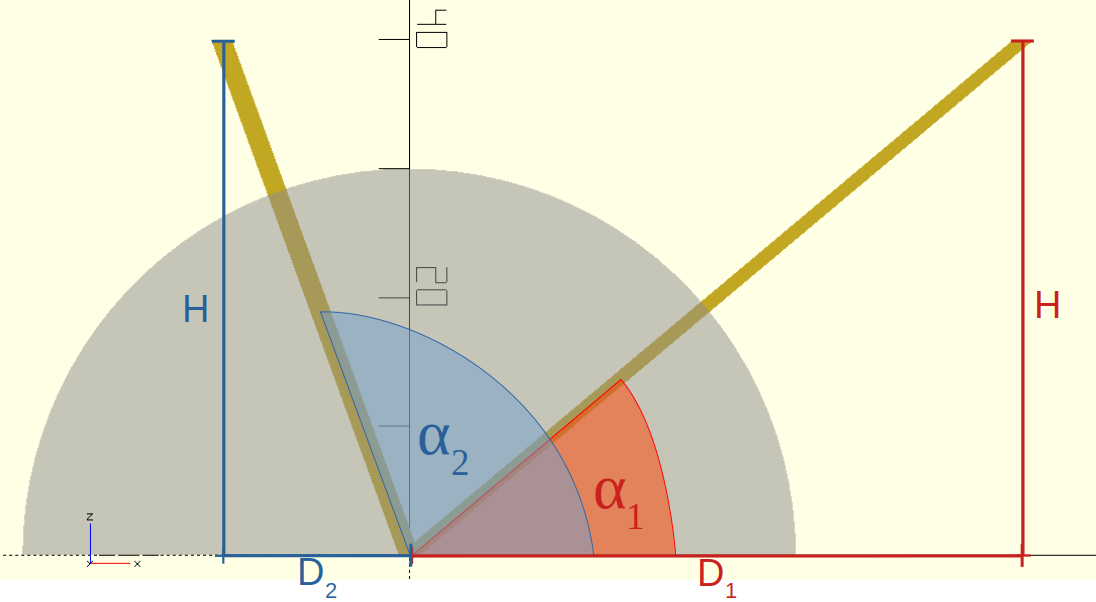
\includegraphics[width=.6\textwidth]{imagenes/dos-rayos-anotados}
  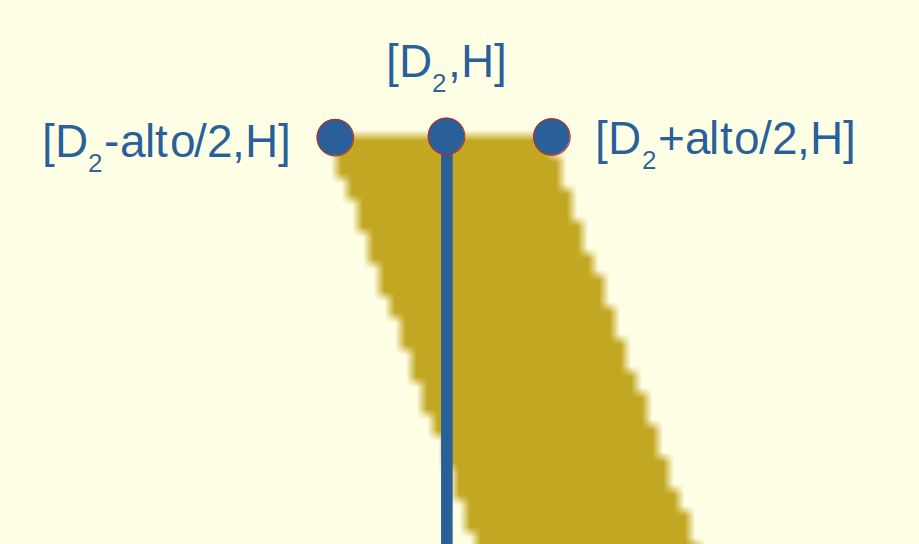
\includegraphics[width=.49\textwidth]{imagenes/haz-alfa2}\hfill
  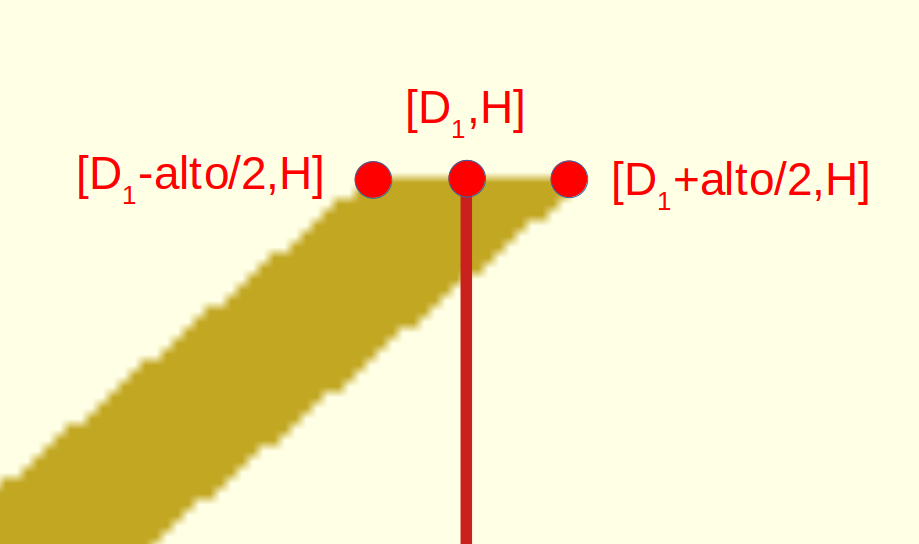
\includegraphics[width=.49\textwidth]{imagenes/haz-alfa1}  
  \caption{Coordenadas superiores del haz de rayos de Sol.}
  \label{fig:dos-rayos-anotados}
\end{figure}

Cecilia no pudo aguantar más:

---¡Pará! ¡Dejame pensar!  ---prorrumpió, y Antonia hizo silencio
bruscamente. Revisó las páginas anteriores junto a la nueva figura
\ref{fig:dos-rayos-anotados}; comprobó que los vértices de la base del
nuevo haz seguían siendo \texttt{[-alto/2,0]} y
\texttt{[alto/2,0]}. Por su parte, los vértices superiores debían
coincidir con los extremos de los dos rayos exteriores del haz:
\texttt{[D$_2$-alto/2,H]} y \texttt{[D$_1$+alto/2,H]}. $D_1$ y $D_2$
sabía cómo calcularlos: el primero era igual a
$\frac{H}{\tan (\alpha_1)}$ y el segundo, análogamente, a
$\frac{H}{\tan (\alpha_2)}$.

Sin demasiada seguridad, debida seguramente al cansancio inducido por
la tortuosa explicación de Antonia más que a cualquier otra cosa,
buscó confirmación con una pregunta tentativa:

---¿Puede ser que el polígono del haz completo se defina con el vector
\texttt{[[-alto/2,0], [D$_2$-alto/2,H], [D$_1$+alto/2,H], [alto/2, 0]]}?

  ---¡¡¡Sí!!! ---gritó Antonia, y hasta \director{} debió haberse
  enterado.

\section{El rayo de Sol revisitado}

Cecilia volvió su mirada sobre el módulo \lstinline!rayo_de_sol!
original:

\begin{lstlisting}
module rayo_de_sol(alfa){
  D=H/tan(alfa);
  vertices=[[-alto_pixel/2,0],
            [D-alto_pixel/2,H],
            [D+alto_pixel/2,H],
            [alto_pixel/2,0]];
  // TODO: medir la duracion de esta solucion
  //       y la de esta otra:
  //       translate([0,ancho_pixel/2,0])
  //       Ojo : borrar 'center=true' abajo
  rotate ([90,0,0])
    linear_extrude(ancho_pixel,center=true)
      polygon(vertices);
}
\end{lstlisting}

No le pareció muy difícil introducir los nuevos cambios, al tiempo que
modificaba el nombre del módulo:

\begin{lstlisting}
module haz_de_sol(alfa1,alfa2){
  D1=H/tan(alfa1);
  D2=H/tan(alfa2);
  vertices=[[-alto_pixel/2,0],
            [D2-alto_pixel/2,H],
            [D1+alto_pixel/2,H],
            [alto_pixel/2,0]];
  // TODO: medir la duracion de esta solucion
  //       y la de esta otra:
  //       translate([0,ancho_pixel/2,0])
  //       Ojo : borrar 'center=true' abajo
  rotate ([90,0,0])
    linear_extrude(ancho_pixel,center=true)
      polygon(vertices);
}
\end{lstlisting}

En la línea 1 dejó lugar para recibir dos ángulos: $\alpha_1$ y
$\alpha_2$. En las líneas 2 y 3 calculaba, con ellos, $D_1$ y
$D_2$. Por último, los vértices de los extremos superiores quedaban
expresados en las líneas 5 y 6. Lo demás, para su sorpresa, quedaba
intacto. Aunque, claro, inmediatamente se dio cuenta de que el cambio
introducido en este módulo impactaría en todos los que se basaban en
él: es decir, prácticamente en todos.

---¿Ahora debemos modificar también el módulo \lstinline!digito!, no?
---preguntó con la voz quebrada: ya se veía reescribiendo todo el
texto completo.

---Sí ---respondió Antonia procurando sonar
tran\-qui\-li\-za\-do\-ra---; pero no te preocupes: verás que todos
los cambios serán así de sencillos. La lógica que pusimos por escrito
en estos módulos está esencialmente bien; sólo debemos ampliarla un
poco ---y tras un instante, pareció querer aprovechar la ocasión para
otra de sus apologías---. Esto es algo que comprobarás que te ocurre
seguido --por no decir siem\-pre-- al escribir un texto un poco
complejo: cuando lo termines advertirás que sólo arribaste a una
primera versión, que necesita --¡y me\-re\-ce!-- una reescritura. Y
eso se debe fundamentalmente a que una nunca escribe un problema
cuando lo entiende, sino que lo entiende cuando lo escribe.

Antonia se detuvo un momento, sin duda para dar tiempo a Cecilia a
saborear la paradoja que sentía que acababa de ofrecer, pero también
como si buscara la mejor manera de continuar, o tratara de evocar y
resumir todos sus recuerdos al respecto:

---Lo que quiero decir es que una de las cosas más lindas de este
género literario es que te ayuda a pensar; aclara tus ideas, o incluso
las crea directamente. Una no escribe para poner en letras de molde
sus ideas: una escribe para pensar, para \emph{tener} ideas. Por eso
la primera escritura de un código nunca puede ser definitiva: es
siempre un primer borrador.

A Cecilia este panegírico no le pareció insensato: ella también había
podido notar, a medida que escribía sus monografías de investigación
astronómica, que las ideas sobre el tema que estudiaba se aclaraban e
incluso surgían a expensas precisamente de la escritura. De pronto se
sintió aún más cerca de Antonia que antes.


\section{El dígito solar revisitado}

Cecilia volvió ahora sobre el módulo \lstinline!digito! original:

\begin{lstlisting}
module digito(alfa,numero){
  for(i=[0:5],j=[0:3]){
    digito=digitos[numero];
    if(digito[i][j]==1){
      x=(i-2.5)*(alto_pixel+delta_alto);
      y=(j-1.5)*(ancho_pixel+delta_ancho);
      translate([x,y,-0.01])
        rayo_de_sol(alfa);
    }
  }
}
\end{lstlisting}

Después de leerlo varias veces, casi no pudo creer que sólo debiera
introducir dos ligerísimos cambios:

\begin{lstlisting}
module digito(numero,alfa1,alfa2){
  for(i=[0:5],j=[0:3]){
    digito=digitos[numero];
    if(digito[i][j]==1){
      x=(i-2.5)*(alto_pixel+delta_alto);
      y=(j-1.5)*(ancho_pixel+delta_ancho);
      translate([x,y,-0.01])
        haz_de_sol(alfa1,alfa2);
    }
  }
}
\end{lstlisting}

Las modificaciones se limitaban a las líneas 1 y 8: la única
responsabilidad del módulo consistía en elegir los pixeles a horadar y
sólo necesitaba los ángulos para pasárselos al módulo
\lstinline!haz_de_sol!.

\section{La hora solar revisitada}

El optimismo de Cecilia iba en aumento; con renovada confianza se
lanzó sobre el módulo \lstinline!hora_solar!:

\begin{lstlisting}
module hora_solar(horas,minutos){
  hora=horas+minutos/60;
  assert(hora>6 && hora<18,"La hora debe encontrarse entre las 6:00 y las 18:00.");
  alfa=alfa(hora);
  hora_decenas=n_a_digito(horas,1);
  hora_unidades=n_a_digito(horas,0);
  minuto_decenas=n_a_digito(minutos,1);
  minuto_unidades=n_a_digito(minutos,0);                    
  delta_y=ancho_pixel+delta_ancho;
  // horas    
  if (hora_decenas != 0)
    translate([0,-8.5*delta_y,0])
      digito(alfa,hora_decenas);
  translate([0,-3.5*delta_y,0])
    digito(alfa,hora_unidades);  
  // minutos
  translate([0,3.5*delta_y,0])
    digito(alfa,minuto_decenas);
  translate([0,8.5*delta_y,0])
    digito(alfa,minuto_unidades);  
  // separador
  separador(horas,minutos);
}
\end{lstlisting}

A medida que lo recorría con la mirada, su sonrisa fue congelándose
hasta convertirse en una mueca de desconcierto. No tardó mucho en
descubrir que había tropezado con un problema fundamental:

---Antonia, este módulo se basa en la idea de perforar el reloj con
una hora \emph{completa}: las 12:00, las 9:40, o la que sea. Pero
nosotras ahora decidimos que sería mejor escribir el cero final de los
minutos de una sola vez, desde las 6:20 a las 17:40, mientras el resto
de los dígitos avanza por su cuenta ---y al tiempo que decía esto, percibió
que el problema se diversificaba aún más---: de hecho, \emph{cada
  dígito} avanza a su propio y distinto ritmo: las decenas de los
minutos lo hacen cada 20, las unidades de las horas cada hora, y las
decenas de las horas sólo toman un valor: el `1', y entre las 10:00 y
las 17:40.

Tras unos instantes en los que buscó inútilmente en el gesto de su
amiga alguna pista, preguntó alarmada:

---¿Debemos deshacernos de este módulo enteramente?

Antonia sonrió:

---Yo creo que no: me parece que es un lindo detalle permitir al
eventual lector o lectora de este texto que imprima un reloj donde
sólo consten algunas horas puntuales que le resulten
significativas. Así, podría tener un reloj que sólo indique las 9:37,
11:41 y 16:22, por ejemplo. Imaginemos que, tal vez, esas horas
particulares tengan un sentido especial para él o para ella.

A Cecilia le pareció una posibilidad muy extravagante; pero supuso
también que un módulo más en el texto no podía arruinarlo ni abarrotar
el espacio de ningún dispositivo de almacenamiento, por lo que podían
en todo caso convivir con él.

---Las modificaciones a este módulo, entonces, son elementales también
---anticipó Antonia, tomando ahora para sí el teclado.

\begin{lstlisting}
module hora_solar(horas,minutos){
  hora=horas+minutos/60;
  assert(hora>6 && hora<18,"La hora debe encontrarse entre las 6:00 y las 18:00.");
  alfa=alfa(hora);
  hora_decenas=n_a_digito(horas,1);
  hora_unidades=n_a_digito(horas,0);
  minuto_decenas=n_a_digito(minutos,1);
  minuto_unidades=n_a_digito(minutos,0);                    
  delta_y=ancho_pixel+delta_ancho;
  // horas    
  if (hora_decenas != 0)
    translate([0,-8.5*delta_y,0])
      digito(hora_decenas,alfa,alfa);
  translate([0,-3.5*delta_y,0])
    digito(hora_unidades,alfa,alfa);  
  // minutos
  translate([0,3.5*delta_y,0])
    digito(minuto_decenas,alfa,alfa);
  translate([0,8.5*delta_y,0])
    digito(minuto_unidades,alfa,alfa);  
  // separador
  separador(hora,minutos);
}
\end{lstlisting}

Cecilia comprobó inmediatamente que todo se limitaba a crear ---en las
líneas 13, 15, 18 y 20--- dígitos cuyos ángulos inicial y final
coincidieran: de esa manera, el haz se convertía naturalmente en el
rayo original. Sonrió con una extraña satisfacción: evidentemente, la
lógica que habían conquistado en un principio seguía funcionando; un
rayo de Sol era, apenas, un caso particular de haz en el que los
ángulos extremos coincidían. Cecilia recuperó de pronto su buen humor.

---Eso sí: fijate en la línea 22. Debemos modificar también el módulo
\lstinline!separador! ---advirtió Antonia, mientras lo señalaba con el
mentón.

\section{El separador revisitado}

\begin{lstlisting}
module separador(horas,minutos){
  alfa=alfa(horas+minutos/60);
  for(i=[-1,1])
    translate([i*0.5*(alto_pixel+delta_alto), 0, -.01])
      rayo_de_sol(alfa);
}
\end{lstlisting}

Cecilia estaba dispuesta a realizar otro cambio trivial, cuando
advirtió que la cosa no era tan sencilla. El módulo esperaba como
parámetros la hora y los minutos: eso funcionaba muy bien para un
separador \emph{instantáneo}, pero no para un separador que tuviera
que extenderse entre dos horarios distintos. Para dar cuerpo a sus
ideas, escribió una rápida modificación.

\begin{lstlisting}
module separador(hora_inicial,
                 minutos_inicial,
                 hora_final,
                 minutos_final){
  alfa1=alfa(hora_inicial+minutos_inicial/60);
  alfa2=alfa(hora_final+minutos_final/60);
  for(i=[-1,1])
    translate([i*0.5*(alto_pixel+delta_alto), 0, -.01])
      haz_de_sol(alfa1,alfa2);
}
\end{lstlisting}

---¿Qué te parece así? ---preguntó, buscando la opinión de su amiga.

Antonia no parecía muy convencida:

---Funciona, por supuesto. Lo que no me convence del todo es que los
dígitos reciben como parámetros $\alpha_1$ y $\alpha_2$, calculados
previamente por otro módulo a partir de las horas correspondientes:
algo me dice que el separador debería adherir a la misma convención
---y escribió su propia versión.

\begin{lstlisting}
module separador(alfa1,alfa2){
  for(i=[-1,1])
    translate([i*0.5*(alto_pixel+delta_alto), 0, -.01])
      haz_de_sol(alfa1,alfa2);
}
\end{lstlisting}

\guillemotright En principio, de esta manera el módulo
\lstinline!hora_solar!  es fácil de adaptar; sólo hay que cambiar la
línea 22 ---agregó Antonia.

\begin{lstlisting}
module hora_solar(horas,minutos){
  hora=horas+minutos/60;
  assert(hora>6 && hora<18,"La hora debe encontrarse entre las 6:00 y las 18:00.");
  alfa=alfa(hora);
  hora_decenas=n_a_digito(horas,1);
  hora_unidades=n_a_digito(horas,0);
  minuto_decenas=n_a_digito(minutos,1);
  minuto_unidades=n_a_digito(minutos,0);                    
  delta_y=ancho_pixel+delta_ancho;
  // horas    
  if (hora_decenas != 0)
    translate([0,-8.5*delta_y,0])
      digito(hora_decenas,alfa,alfa);
  translate([0,-3.5*delta_y,0])
    digito(hora_unidades,alfa,alfa);  
  // minutos
  translate([0,3.5*delta_y,0])
    digito(minuto_decenas,alfa,alfa);
  translate([0,8.5*delta_y,0])
    digito(minuto_unidades,alfa,alfa);  
  // separador
  separador(alfa,alfa);
}
\end{lstlisting}

A Cecilia no le costó nada estar de acuerdo.

---Muy bien ---resumió Antonia con una sonrisa satisfecha, y
reclinándose contra la silla mientras contemplaba el texto sin
disimular una nota de orgullo en su voz---. Acabamos de lograr algo
muy importante: reescribimos el código original de forma más general,
sin que por eso deje de funcionar en el caso particular que veníamos
trabajando: horas y minutos puntuales.


\begin{lstlisting}
module reloj_de_sol(){
  difference(){
    cuerpo(largo_reloj);    
    hora_solar(12,0);
    hora_solar(15,40);
  }
}
reloj_de_sol();
\end{lstlisting}%


\begin{figure}[ht]
  \centering
  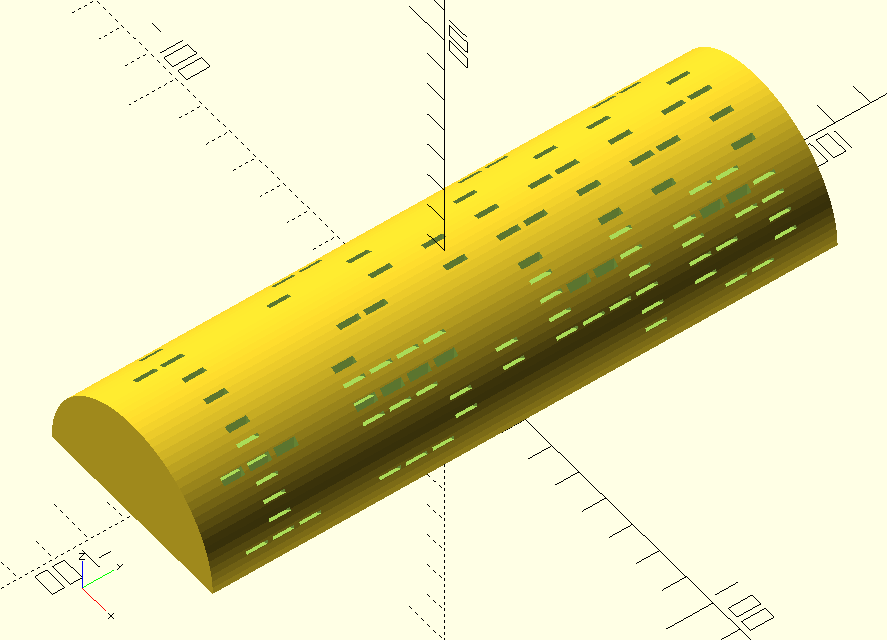
\includegraphics[width=\textwidth]{imagenes/dos-horas-optimizadas}
  \caption{Dos horas puntuales logradas con el nuevo texto
    optimizado, lo que demuestra que la refactorización del mismo no
    afectó su funcionalidad original.}\iftoggle{libro}{\vspace{128in}}{}
  \label{fig:dos-horas-optimizadas}
\end{figure}

---Si no me equivoco, los angloparlantes llaman a este proceder
\emph{refactoring}\footnote{Tiene equivalencia en castellano, y no
  suena tan mal: \emph{refactorización}. (nota del Editor)} ---agregó
Antonia.

---¿Me prometés que en el capítulo siguiente terminamos el reloj?
---suplicó Cecilia, que tras
\pagedifferenceplusone{sec:el-reloj-de-sol-iii}{sec:el-reloj-de-sol-iii-b}
páginas ya no quería otra cosa que
descansar.\label{sec:el-reloj-de-sol-iii-b}

---Te lo prometo ---concedió su amiga---. Al menos la cuestión central
de las horas y los minutos. En el capítulo \ref{sec:texto} quiero
mostrarte cómo agregar texto tridimensional a los objetos: un reloj de
Sol sin leyendas no es un reloj de Sol.

Cecilia recordaba esa otra promesa, y esperaba que esta vez Antonia
cumpliera ambas a la brevedad.


%%% Local Variables:
%%% mode: latex
%%% TeX-master: "../libro"
%%% End:
